\documentclass{beamer}
\usetheme{Boadilla}
\usecolortheme{dolphin}
\usefonttheme{serif}
\setbeamertemplate{navigation symbols}{}
\setbeamertemplate{caption}[numbered]
\usepackage{graphicx}
\usepackage{amsmath}
\usepackage{hyperref}
\usepackage{booktabs}
\usepackage{multicol}
\usepackage{pgfplots}
\pgfplotsset{compat=1.18}

\title{An Economic Analysis of Optimal Investment Strategies for Accumulating Housing Down Payments}
\author{Frank Paul Longo II}
\date{\today}

\begin{document}

\begin{frame}
    \titlepage
\end{frame}





\section{Introduction}
\begin{frame}{Introduction}
    \begin{block}{Objective}
        Develop optimal investment strategies for first-time homebuyers to save for down payments.
    \end{block}
    \begin{block}{Research Question}
        What are the optimal investment strategies for aspiring first-time homebuyers of various age cohorts to accumulate down payments over 5, 7.5, and 10-year investment horizons?
    \end{block}
    \begin{block}{Motivation}
        Address the challenges posed by escalating housing costs and help diverse age groups achieve homeownership faster.
    \end{block}
\end{frame}








\section{Typical First-time Homebuyer Profile}
\begin{frame}{Typical First-time Homebuyer Profile}
    \begin{block}{Demographics}
        \begin{itemize}
            \item \textbf{Median Age:} 35 years (2024)\footnote{National Association of Realtors, 2024 Profile of Home Buyers and Sellers.}
            \item \textbf{Median Household Income:} \$104,000 (2024)\footnote{Consumer Financial Protection Bureau, Market Snapshot: First-time Homebuyers, 2024.}
            \item \textbf{Median Nationwide Home Price:} \$416,100 (2024)\footnote{U.S. Department of Housing and Urban Development, 2024.}
        \end{itemize}
    \end{block}
\end{frame}

















\section{Data Import}
\begin{frame}{Data Sources}
    \begin{block}{Primary Sources}
        \textbf{Yahoo Finance (YFinance)}
        \begin{itemize}
            \item Financial data for stocks, mutual funds, and ETFs.
        \end{itemize}
    \end{block}
    \begin{block}{Data Coverage}
        \textbf{YFinance Data}
        \begin{itemize}
            \item \textbf{Date Range:} 2011-05-04 to 2014-11-07 (daily frequency)
        \end{itemize}
        \textbf{Hindsight Data}
        \begin{itemize}
            \item \textbf{Date Range:} 2011-05-04 to 2024-07-9 (daily frequency)
        \end{itemize}
    \end{block}
    \begin{block}{Data Fields}
        \begin{multicols}{2}
        \begin{itemize}
            \item Open
            \item High
            \item Low
            \item Close
            \item Adj Close
            \item Volume
            \item Type
        \end{itemize}
        \end{multicols}
    \end{block}
\end{frame}

\begin{frame}{Distribution of Security Types}
    \begin{figure}
        \centering
        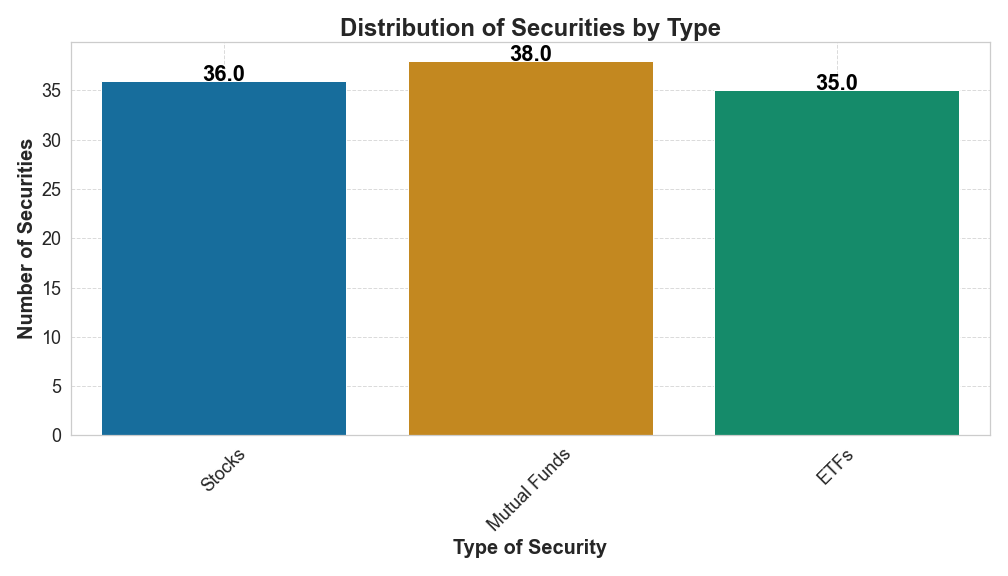
\includegraphics[width=\linewidth]{histogram_security_count.png}
    \end{figure}
\end{frame}

\begin{frame}{Cumulative Returns by Type}
    \begin{figure}
        \centering
        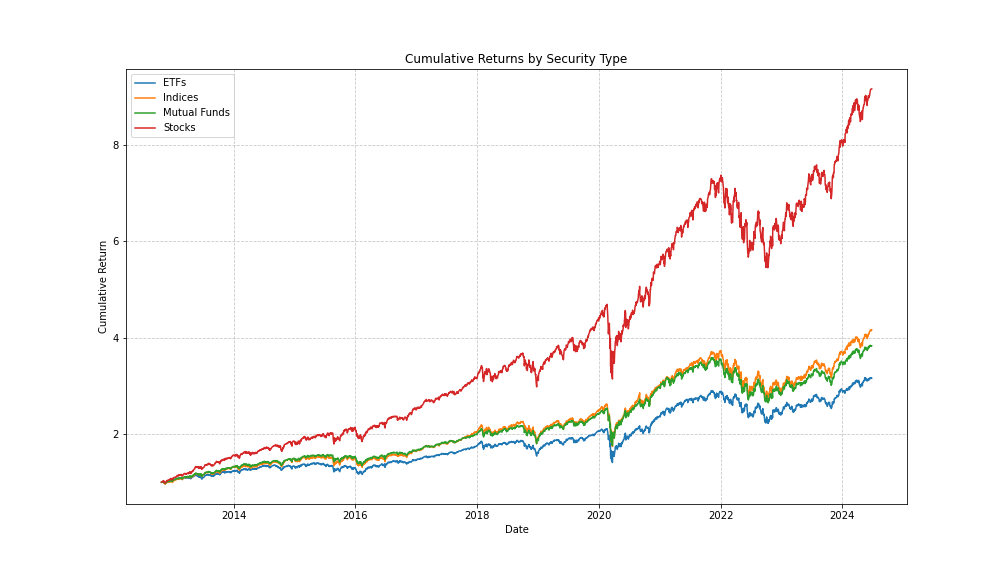
\includegraphics[width=\linewidth]{cumulative_returns_by_type.png}
    \end{figure}
\end{frame}







\section{CAPM}
\begin{frame}{Capital Asset Pricing Model (CAPM)}
    \begin{block}{Formula} 
        \begin{equation*}
            E(R_i) = R_f + \beta_i (E(R_m) - R_f)
        \end{equation*}
        \footnote{Sharpe, W. F. (1964). Capital asset prices: A theory of market equilibrium under conditions of risk. \textit{The Journal of Finance}, 19(3), 425-442.}
    \end{block}
    \begin{block}{Explanation of Variables}
        \begin{itemize}
            \item \( E(R_i) \): Expected return of the investment
            \item \( R_f \): Risk-free rate of return
            \item \( \beta_i \): Beta of the investment, a measure of its volatility relative to the market
            \item \( E(R_m) \): Expected return of the market
            \item \( E(R_m) - R_f \): Market risk premium, the additional return expected from the market above the risk-free rate
        \end{itemize}
    \end{block}
\end{frame}



\begin{frame}{Composite Score Technique}
    \begin{block}{Composite Score Technique}
        \begin{itemize}
            \item Combines Beta, CAPM Predicted Return, Actual Return, and Sharpe Ratio into a single score.
            \item Metrics are normalized and weighted for importance.
            \item Identifies assets offering best risk-adjusted returns over specified time horizons.
        \end{itemize}
    \end{block}
\end{frame}


\begin{frame}{30-35 Years Old (5-Year Time Horizon)}
    \begin{block}{Assigned Metrics and Weights}
        \begin{itemize}
            \item Beta: 0.20
            \item Sharpe Ratio: 0.30
            \item CAPM Predicted Return: 0.20
            \item Actual Returns: 0.30
        \end{itemize}
    \end{block}
    \begin{block}{Assigned Constraints}
        \begin{itemize}
            \item Sharpe Ratio greater than 75th percentile.
            \item Beta less than 1.5.
        \end{itemize}
    \end{block}
\end{frame}

\begin{frame}{25-30 Years Old (7.5-Year Time Horizon)}
    \begin{block}{Assigned Metrics and Weights}
        \begin{itemize}
            \item Beta: 0.20
            \item Sharpe Ratio: 0.25
            \item CAPM Predicted Return: 0.25
            \item Actual Returns: 0.30
        \end{itemize}
    \end{block}
    \begin{block}{Assigned Constraints}
        \begin{itemize}
            \item Sharpe Ratio greater than 50th percentile.
            \item Beta less than 2.0.
        \end{itemize}
    \end{block}
\end{frame}

\section{Risk Tolerances and Investment Contributions}
\begin{frame}{20-25 Years Old (10-Year Time Horizon)}
    \begin{block}{Assigned Metrics and Weights}
        \begin{itemize}
            \item Beta: 0.15
            \item Sharpe Ratio: 0.25
            \item CAPM Predicted Return: 0.25
            \item Actual Returns: 0.35
        \end{itemize}
    \end{block}
    \begin{block}{Assigned Constraints}
        \begin{itemize}
            \item Sharpe Ratio greater than 25th percentile.
            \item Beta less than 2.5.
        \end{itemize}
    \end{block}
\end{frame}




\begin{frame}{Top Assets by Composite Score (5 Years)}
    \begin{figure}
        \centering
        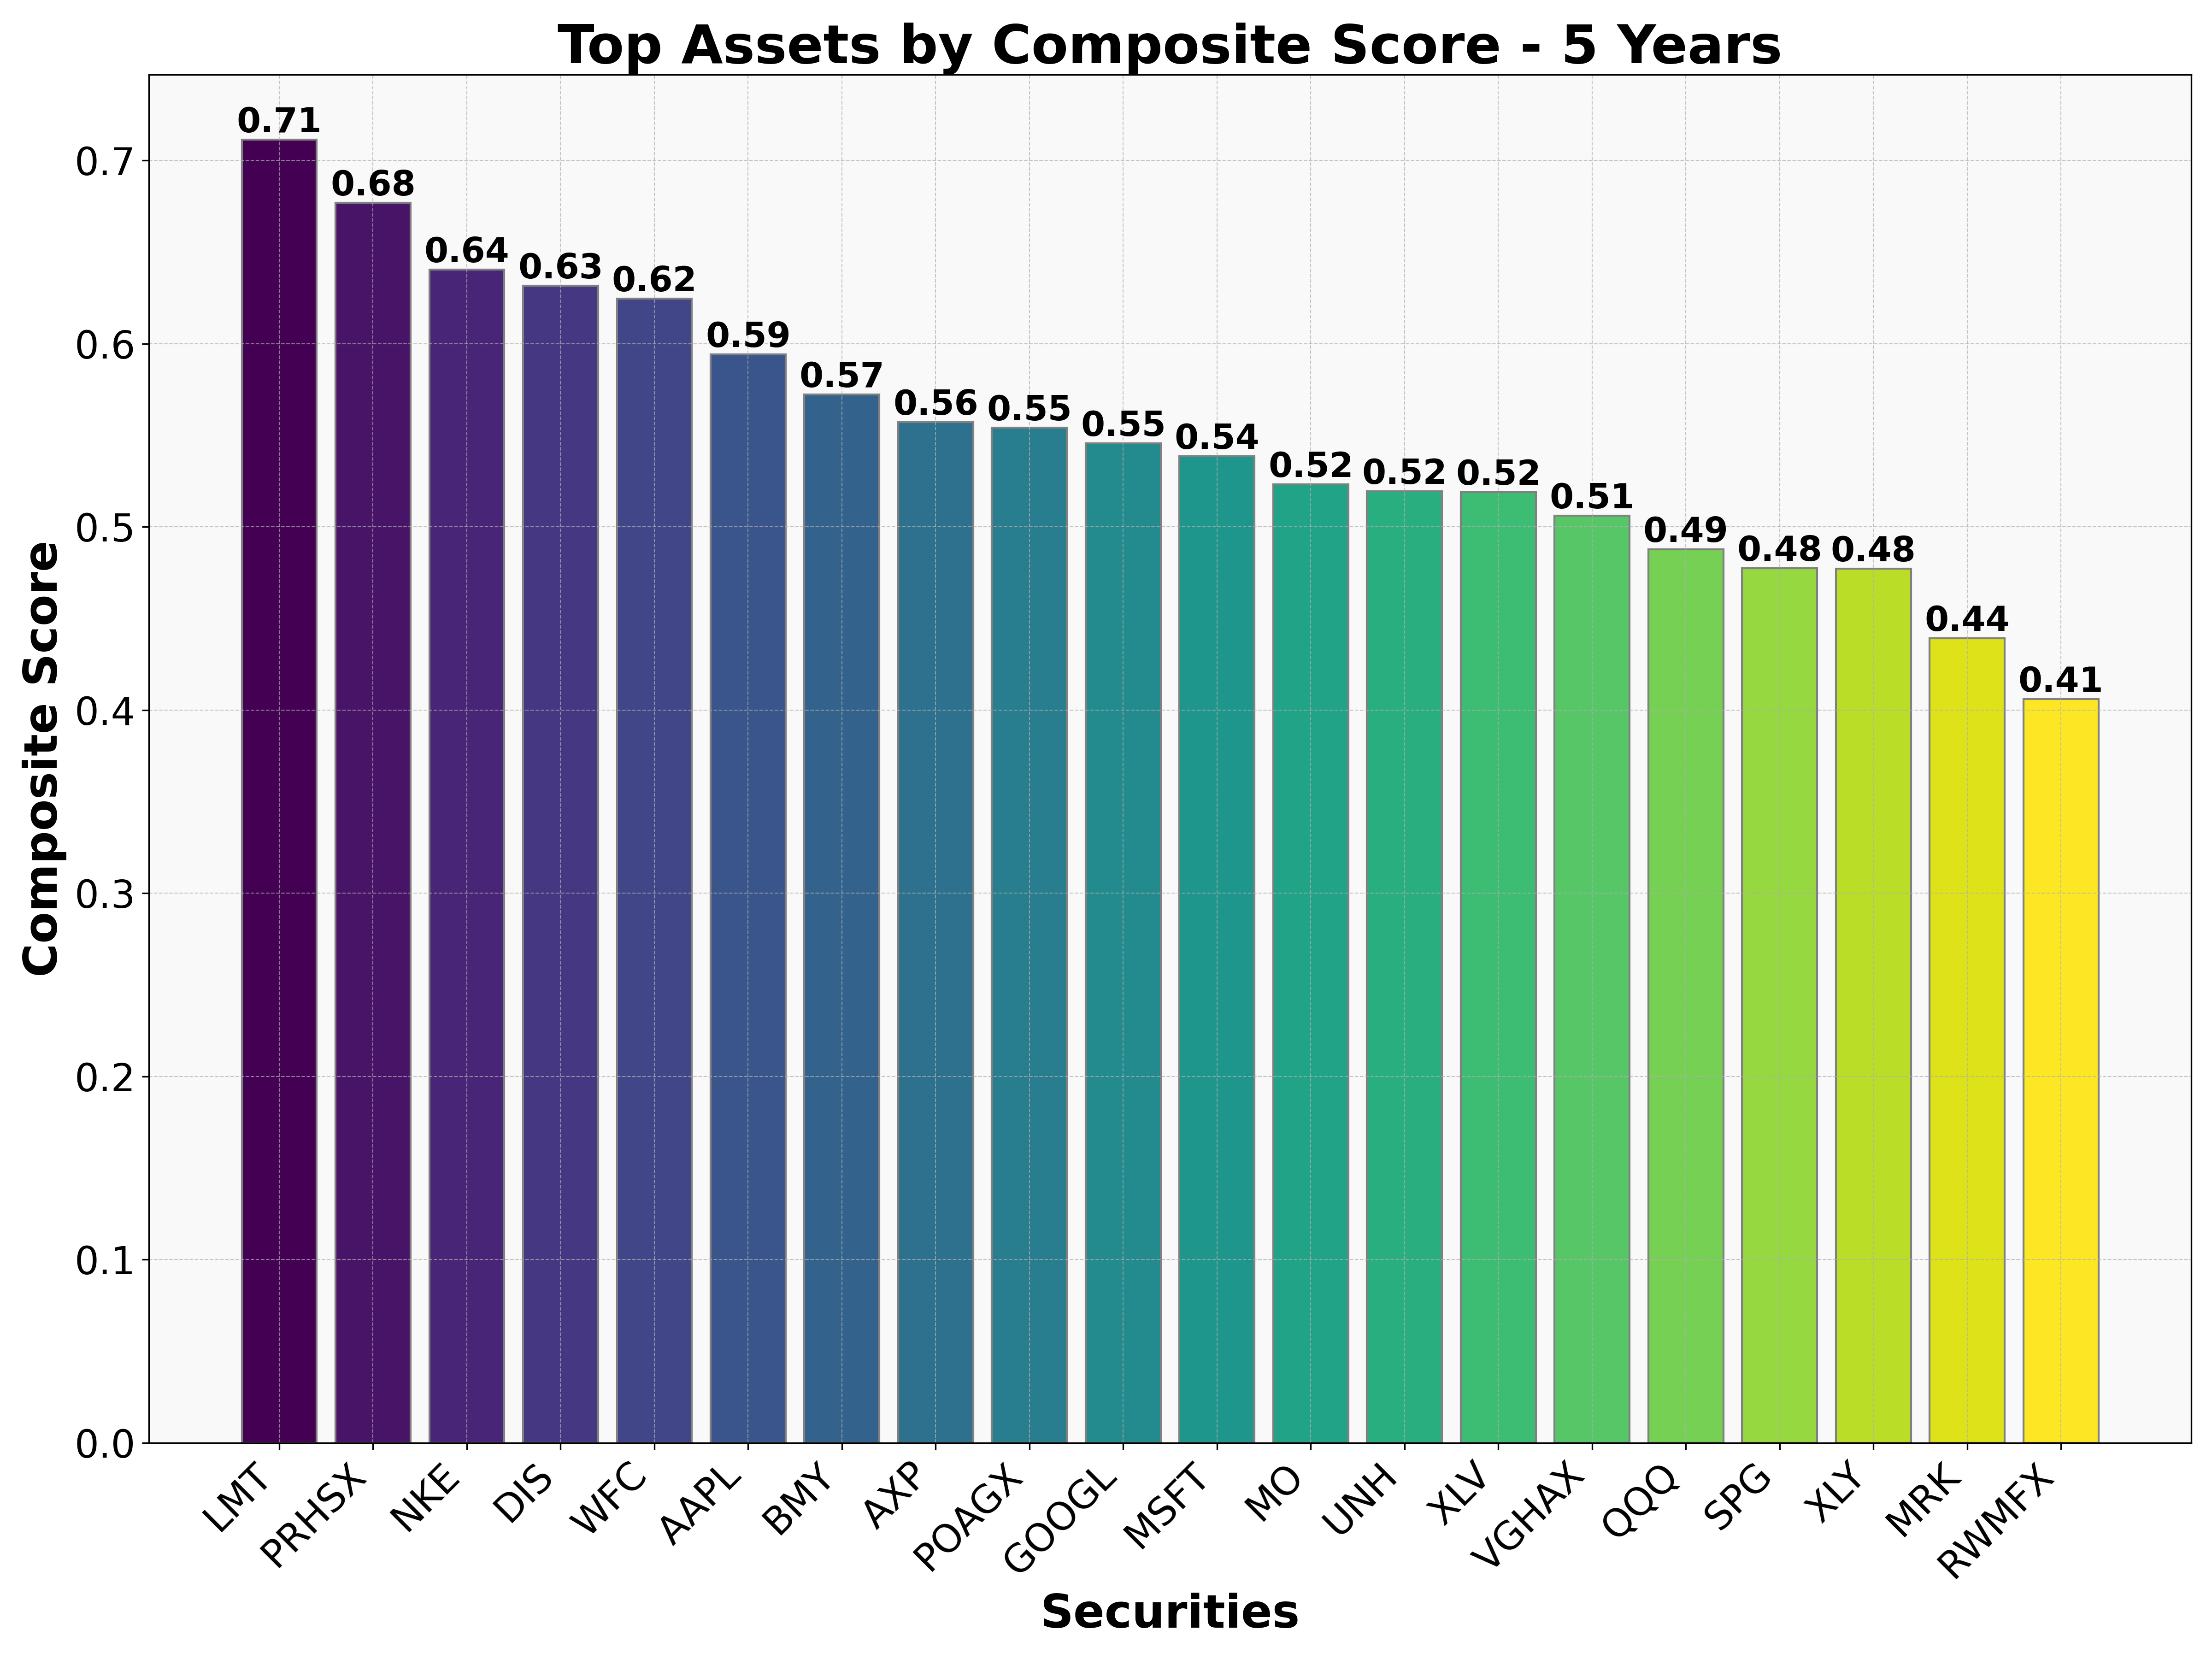
\includegraphics[width=0.9\linewidth]{top_assets_composite_score_5_years.png}
    \end{figure}
\end{frame}

\begin{frame}{Top Assets by Composite Score (7.5 Years)}
    \begin{figure}
        \centering
        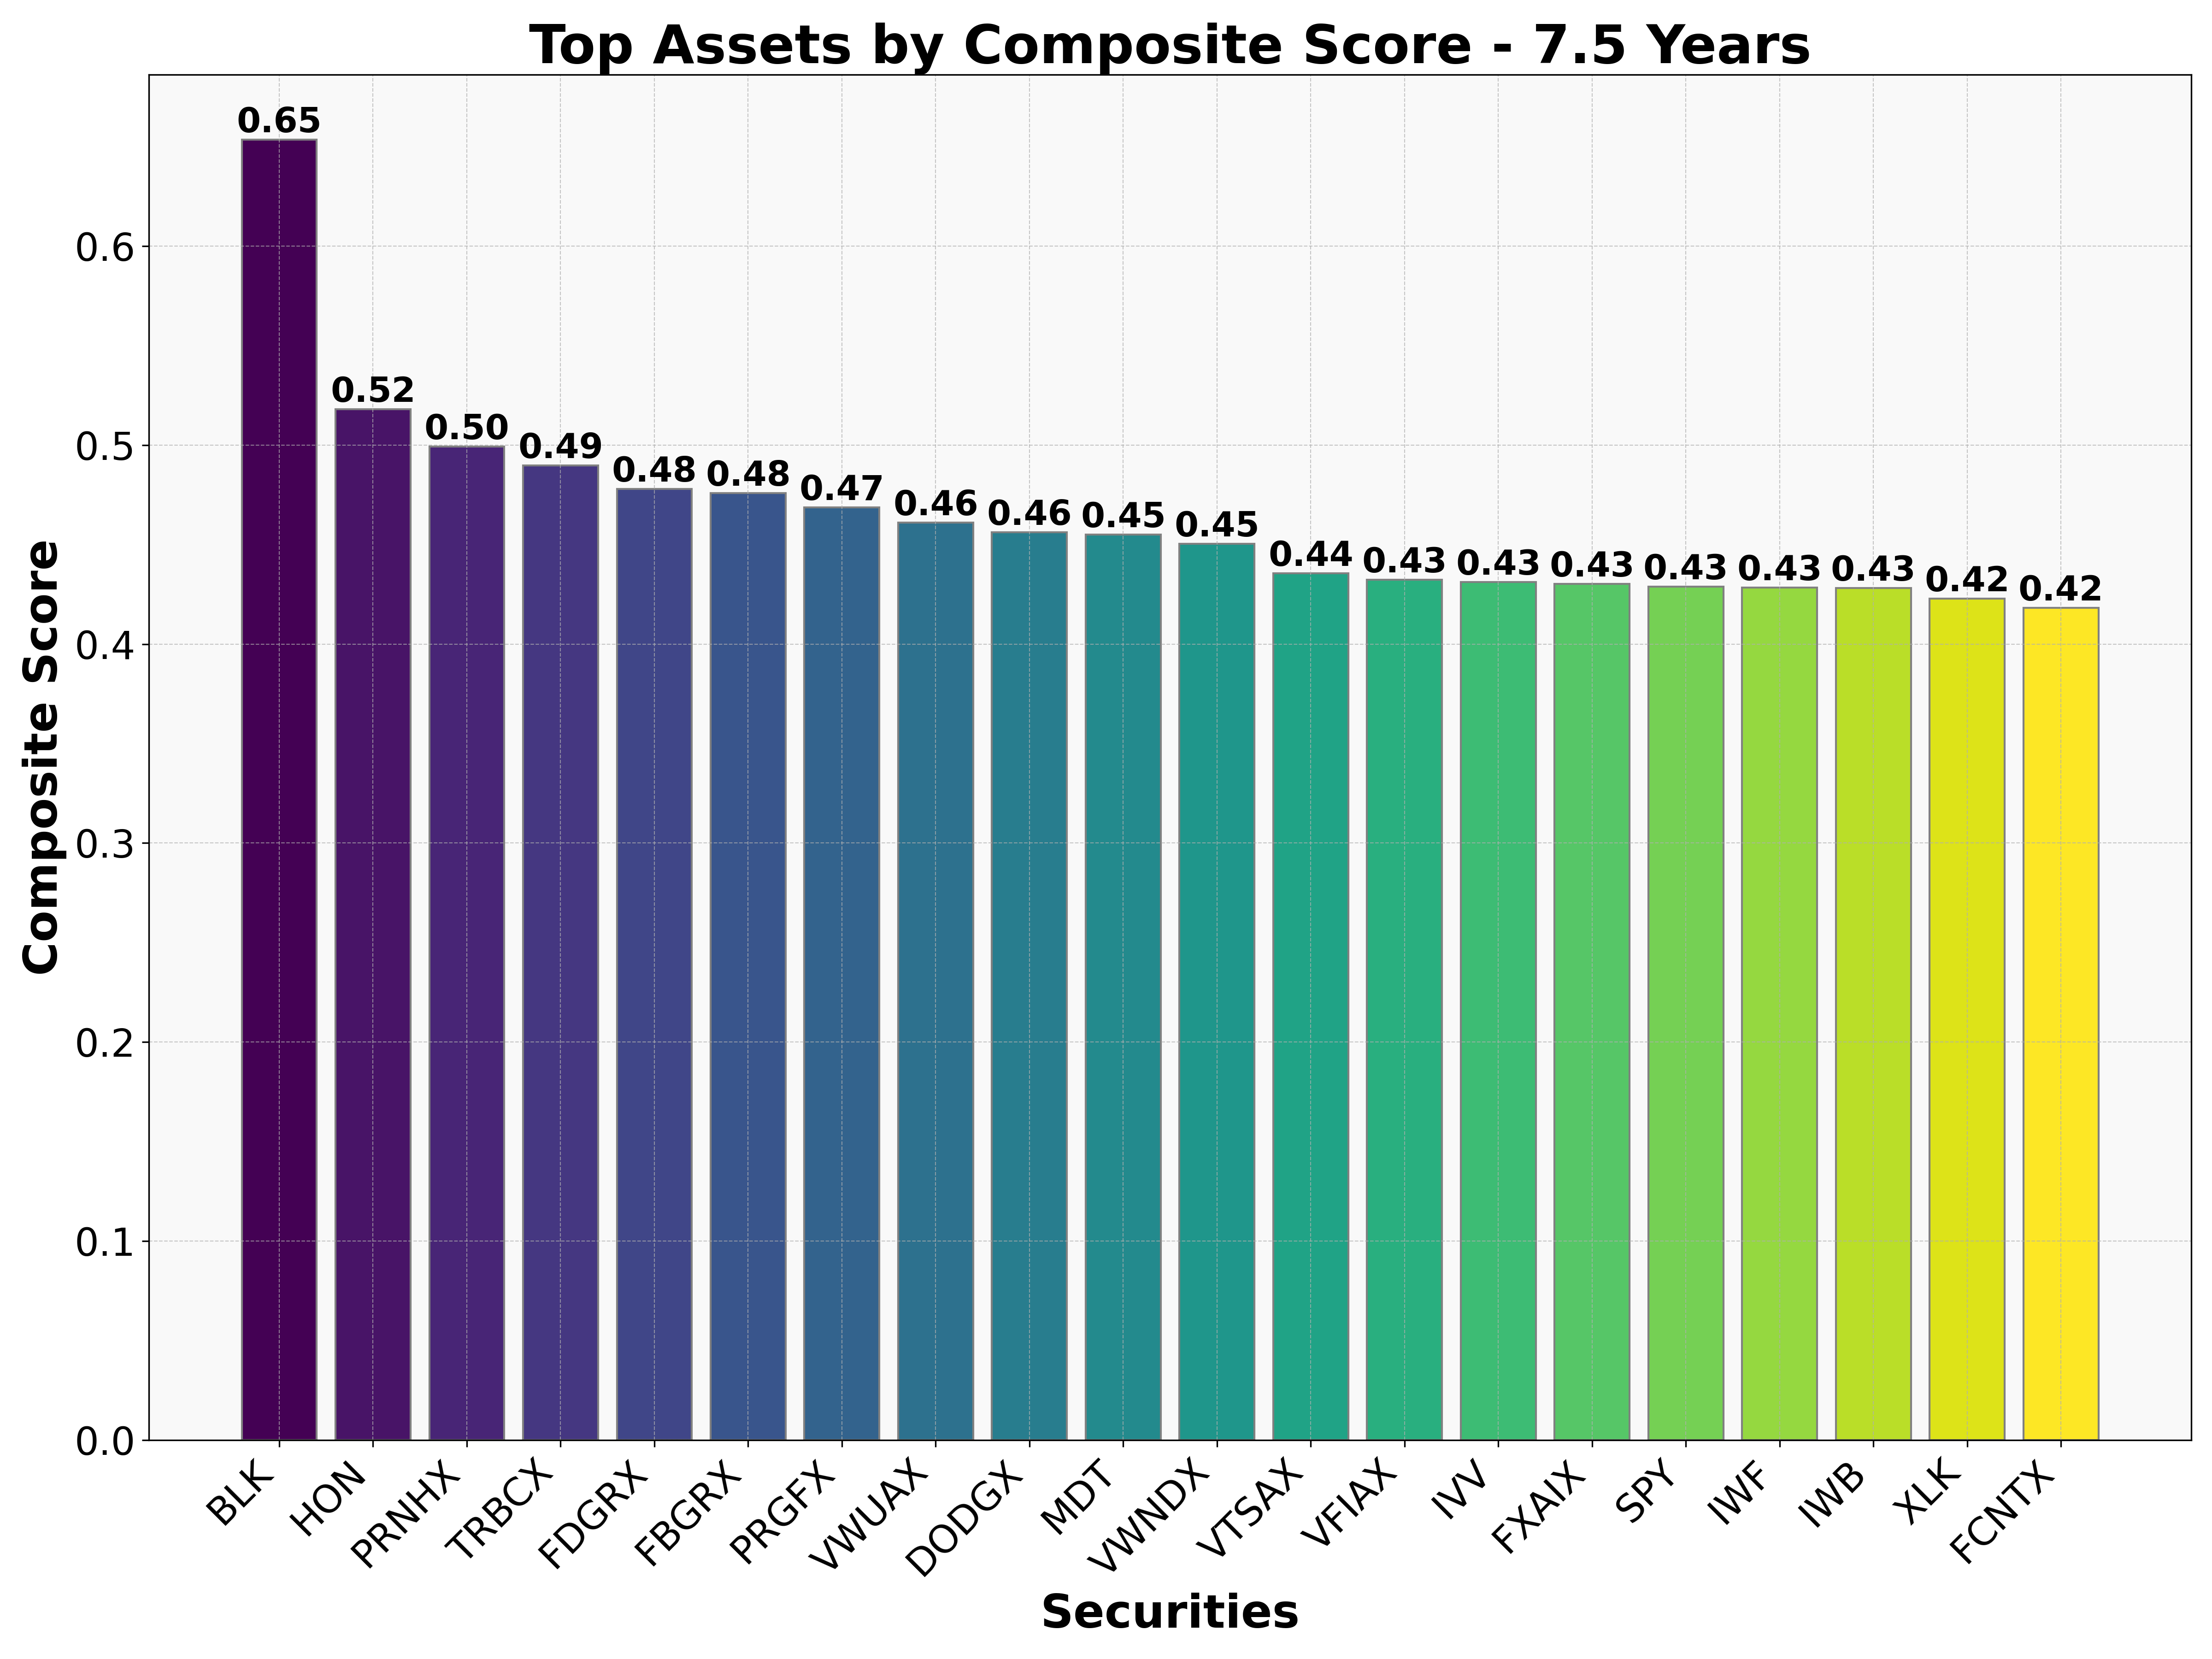
\includegraphics[width=0.9\linewidth]{top_assets_composite_score_7_5_years.png}
    \end{figure}
\end{frame}

\section{Composite Scores}
\begin{frame}{Top Assets by Composite Score (10 Years)}
    \begin{figure}
        \centering
        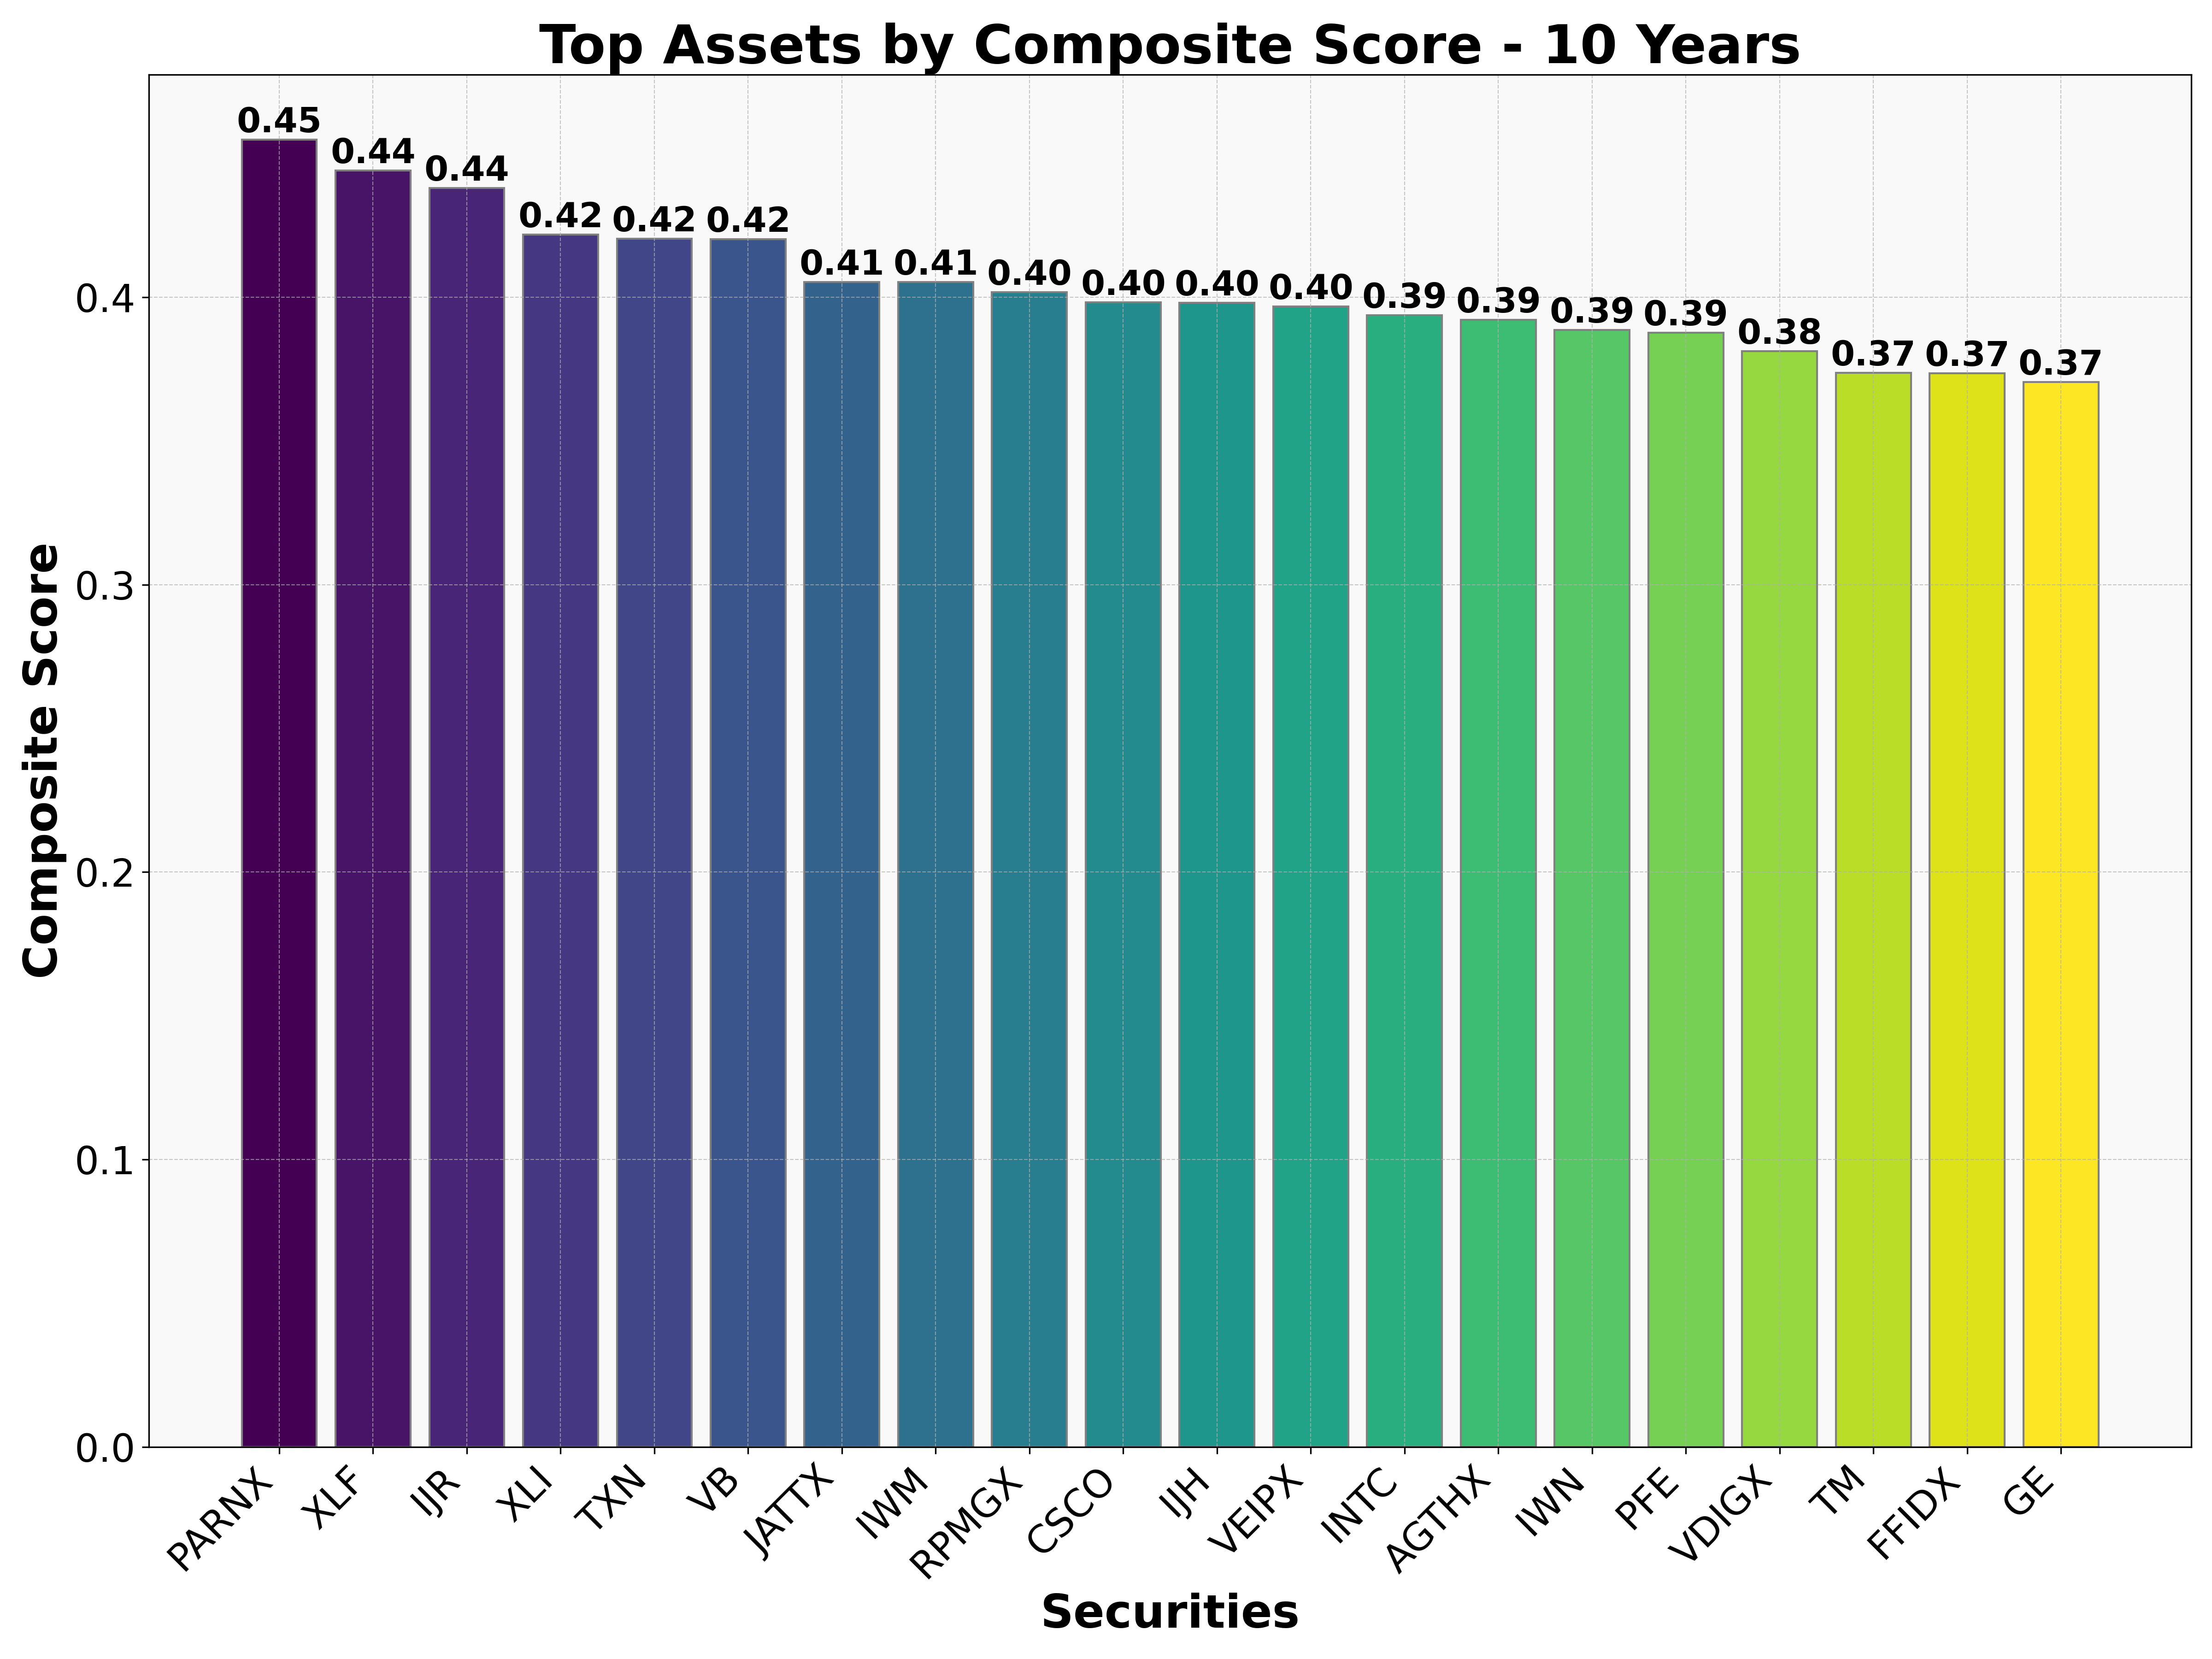
\includegraphics[width=0.9\linewidth]{top_assets_composite_score_10_years.png}
    \end{figure}
\end{frame}











\section{Modern Portfolio Theory (MPT)}
\begin{frame}{Modern Portfolio Theory (MPT)}
    \begin{block}{Overview}
        A framework for constructing a portfolio to maximize return for a given level of risk.\footnote{Markowitz, H. (1952). Portfolio Selection. \textit{The Journal of Finance}, 7(1), 77-91.}
    \end{block}
    \begin{block}{Formulas}
        \begin{equation*}
            \sigma_p^2 = \sum_{i=1}^{n} \sum_{j=1}^{n} w_i w_j \sigma_{ij}
        \end{equation*}
    \end{block}
    \begin{block}{Definitions}
        \begin{multicols}{2}
            \begin{itemize}
                \item \(E(R_p)\): Portfolio return
                \item \(w_i\): Weight of asset \(i\)
                \item \(E(R_i)\): Return of asset \(i\)
                \item \(\sigma_p^2\): Portfolio variance
                \item \(\sigma_{ij}\): Covariance of assets \(i, j\)
            \end{itemize}
        \end{multicols}
    \end{block}
\end{frame}

\begin{frame}{Optimize the Portfolio}
    \begin{block}{Objective}
        Adjust the weights of the assets to maximize the portfolio's expected return for a given level of risk or to minimize risk for a given level of expected return.
    \end{block}
    \begin{block}{Optimization Problem}
        Solve the following optimization problem:
        \begin{equation*}
            \min \sigma_p^2 = \sum_{i=1}^{n} \sum_{j=1}^{n} w_i w_j \sigma_{ij}
        \end{equation*}
        Subject to:
        \begin{equation*}
            \sum_{i=1}^{n} w_i = 1 \quad \text{and} \quad E(R_p) = \sum_{i=1}^{n} w_i E(R_i)
        \end{equation*}
    \end{block}
\end{frame}

\begin{frame}{Optimal Portfolio Calculation}
    \begin{block}{Methodology}
        The optimal weights for the portfolios over different time horizons (5 years, 7.5 years, and 10 years) were calculated using the following steps:
        \begin{itemize}
            \item Historical returns and covariance matrices of the assets were computed.
            \item The optimization problem was solved using numerical methods to find the weights that minimize the portfolio variance for a given expected return.
            \item Constraints were applied to ensure that the sum of the weights equals 1 and that all weights are non-negative.
        \end{itemize}
    \end{block}
\end{frame}

\begin{frame}{Optimal Portfolio (5 Years)}
    \begin{figure}
        \centering
        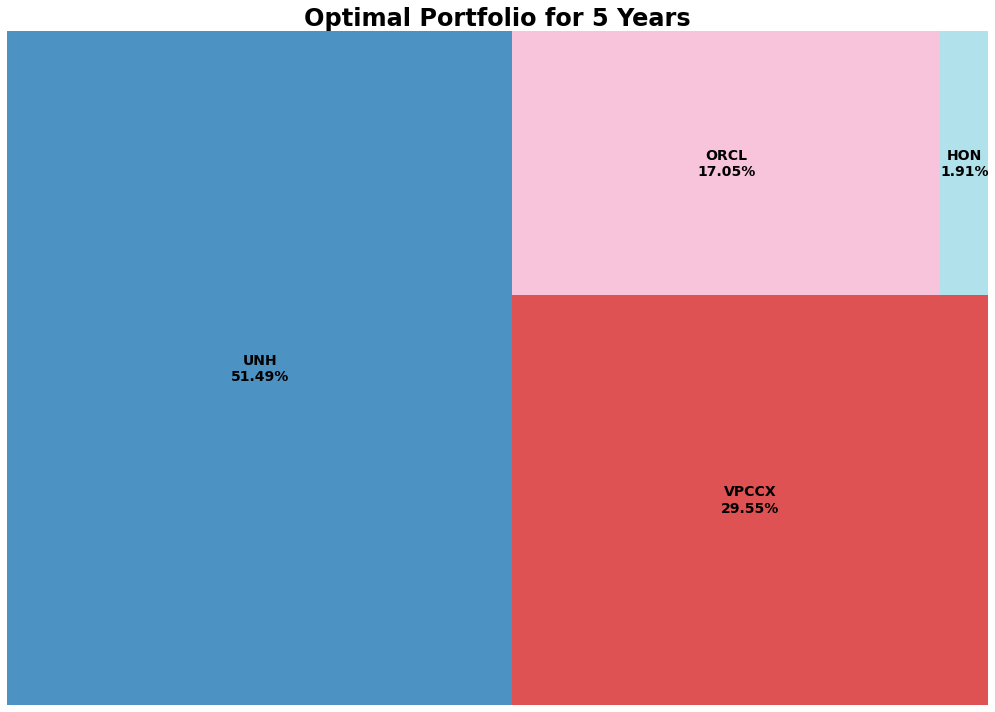
\includegraphics[height=0.8\textheight]{optimal_portfolio_5_years.png}
    \end{figure}
\end{frame}

\begin{frame}{Optimal Portfolio (7.5 Years)}
    \begin{figure}
        \centering
        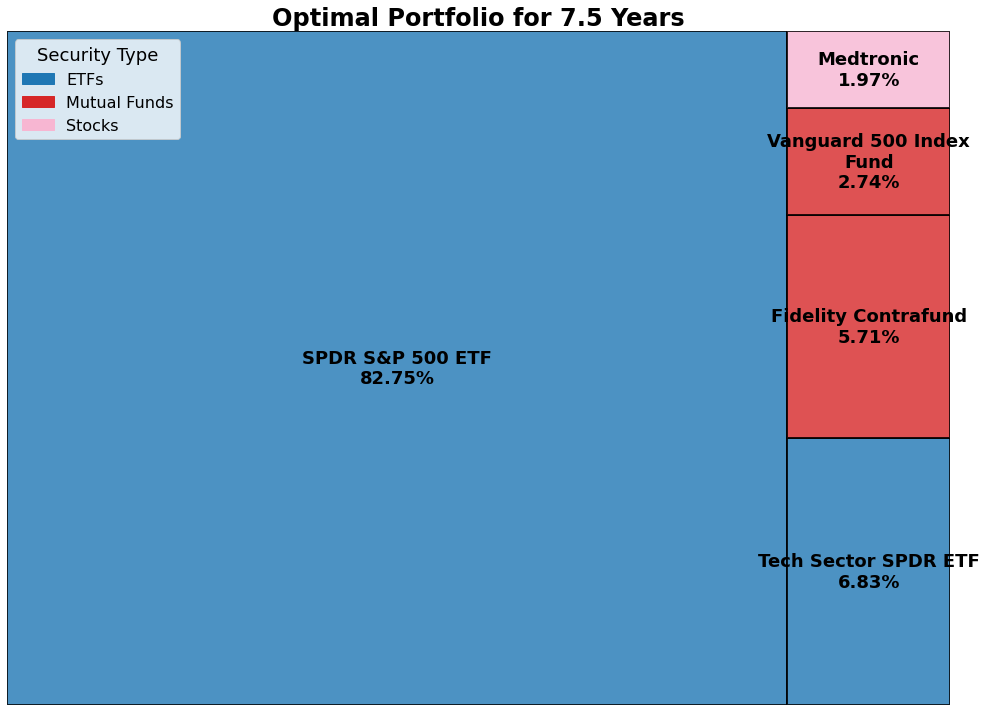
\includegraphics[height=0.8\textheight]{optimal_portfolio_7_5_years.png}
    \end{figure}
\end{frame}

\begin{frame}{Optimal Portfolio (10 Years)}
    \begin{figure}
        \centering
        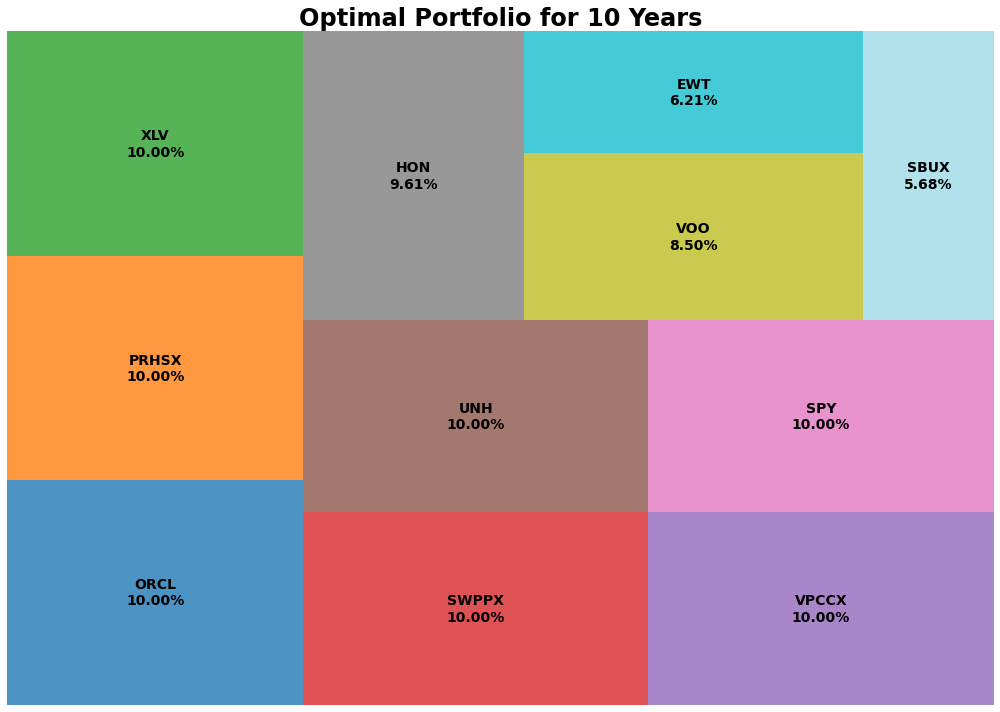
\includegraphics[height=0.8\textheight]{optimal_portfolio_10_years.png}
    \end{figure}
\end{frame}





\section{Performance Analysis of Investment Portfolios}
\begin{frame}
\frametitle{Performance Analysis of Investment Portfolios}
    \begin{block}{Data Sources}
        \begin{itemize}
            \item Historical market data for S\&P 500 and portfolio constituents.
            \item Optimal weights for each horizon portfolio.
        \end{itemize}
    \end{block}
    \begin{block}{Methodology}
        \begin{itemize}
            \item Calculate cumulative returns for each portfolio and compare against the S\&P 500.
            \item Visualize the performance using cumulative return charts.
        \end{itemize}
    \end{block}
\end{frame}


\begin{frame}{Cumulative Returns Comparison}
    \begin{figure}
        \centering
        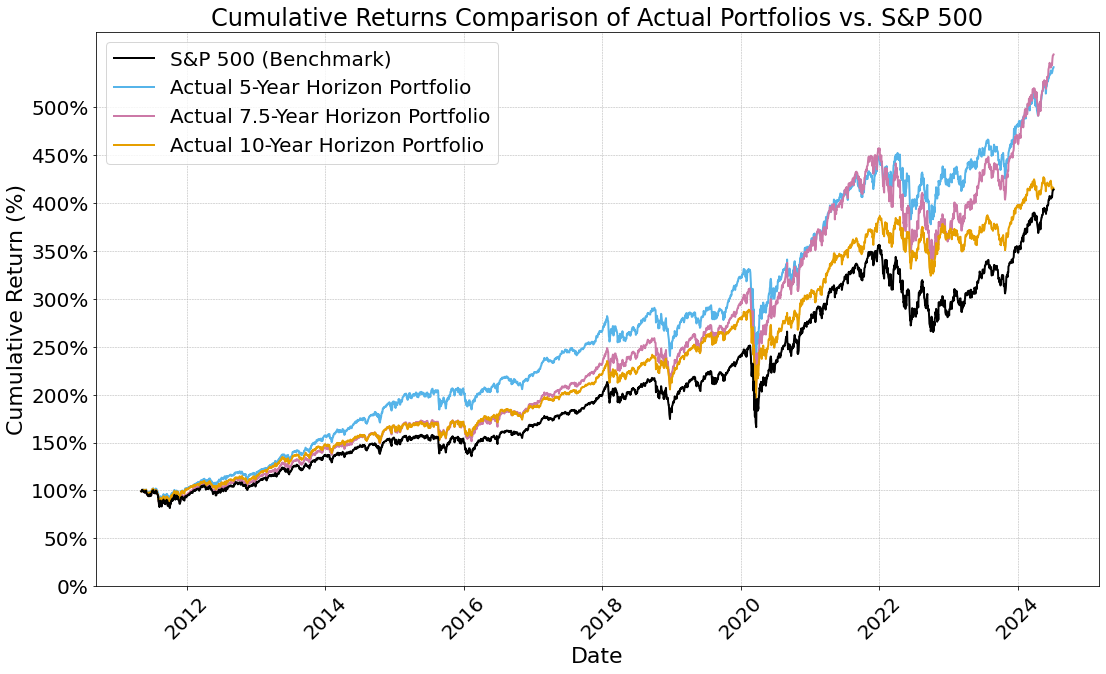
\includegraphics[width=0.9\textwidth]{cumulative_returns_comparison.png}
    \end{figure}
\end{frame}

\begin{frame}{Summary of Cumulative Returns}
    \begin{figure}
        \centering
        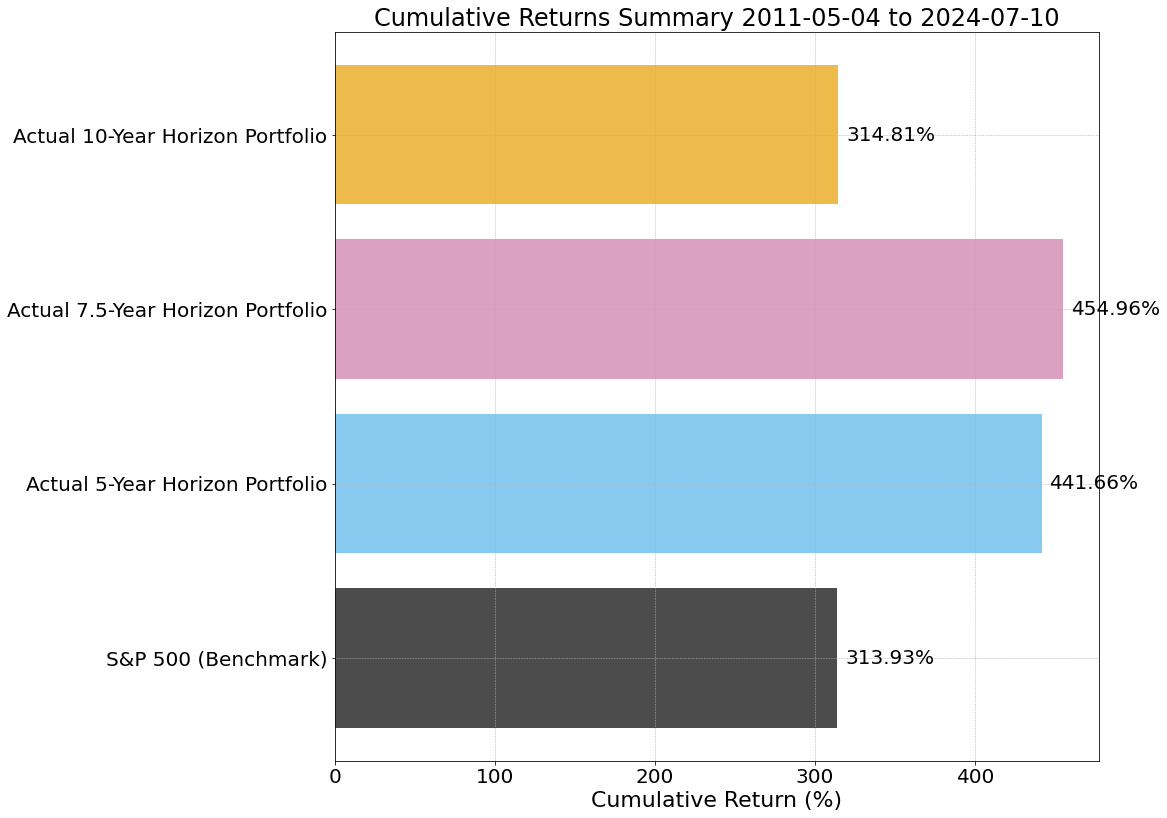
\includegraphics[width=0.9\textwidth]{cumulative_returns_summary.png}
    \end{figure}
\end{frame}

\begin{frame}
\frametitle{Analysis and Insights}
    \begin{block}{Key Observations}
        \begin{itemize}
            \item All horizon portfolios outperformed the S\&P 500 benchmark over the observed period.
            \item The 5-year horizon portfolio performed well with a return of 441.66%.
            \item The 7.5-year horizon portfolio achieved the highest cumulative return of 454.96%.
            \item The 10-year horizon portfolio lagged behind the others with a return of 314.81%.
        \end{itemize}
    \end{block}
\end{frame}






\section{Results Interpretation}
\begin{frame}{Results Interpretation}
    \begin{block}{Findings}
        Through this analysis using the Capital Asset Pricing Model (CAPM) and Modern Portfolio Theory (MPT), we successfully identified the optimal weights for the selected securities. The analysis revealed that diversification across different asset classes and strategic allocation can significantly enhance the potential for accumulating sufficient down payments over varying time horizons.
    \end{block}
    \begin{block}{Implications}
        These findings underscore the importance of tailored investment strategies for different age groups purchasing a home for the first time. By leveraging these models, first-time homebuyers can make informed decisions that align with their financial goals and risk tolerance.
    \end{block}
\end{frame}






\section{References}
\begin{frame}{References (1/2)}
    \begin{block}{}
        \begin{itemize}
            \item Boyle, P. P. (1977). Options: A Monte Carlo Approach. \textit{Journal of Financial Economics, 4}(3), 323-338. DOI: 10.1016/0304-405X(77)90005-8
            \item Federal Reserve. (2023). Report on the Economic Well-Being of U.S. Households in 2023. Retrieved from \url{https://www.federalreserve.gov/publications/2023-economic-well-being-of-us-households-in-2023.htm}
            \item Investment Company Institute. (n.d.). Retrieved from \url{https://www.ici.org/}
            \item Markowitz, H. (1952). Portfolio Selection. \textit{Journal of Finance, 7}(1), 77-91. DOI: 10.2307/2975974
        \end{itemize}
    \end{block}
\end{frame}

\begin{frame}{References (2/2)}
    \begin{block}{}
        \begin{itemize}
            \item Morgan Stanley. (2024). Risk Tolerance Report. Retrieved from \url{https://www.morganstanley.com/}
            \item National Association of Realtors. (2023). 2023 Home Buyer and Seller Generational Trends. Retrieved from \url{https://www.nar.realtor/research-and-statistics/research-reports/home-buyer-and-seller-generational-trends}
            \item Sharpe, W. F. (1964). Capital Asset Prices: A Theory of Market Equilibrium under Conditions of Risk. \textit{The Journal of Finance, 19}(3), 425-442. DOI: 10.2307/2975974
            \item Sharpe, W. F. (1966). Mutual Fund Performance. \textit{Journal of Business, 39}(1), 119-138. DOI: 10.1086/294846
            \item U.S. Department of Housing and Urban Development. (2024). Housing Market Analysis. Retrieved from \url{https://www.hud.gov/}
            \item Yahoo Finance. (n.d.). Retrieved from \url{https://finance.yahoo.com/}
        \end{itemize}
    \end{block}
\end{frame}







\end{document}
